\documentclass{article}

\usepackage[margin=0.5in]{geometry}
\linespread{1.15}
%\setlength{\parskip}{1ex}
%\setlength{\parindent}{0pt}
% \usepackage{parskip}
\usepackage{siunitx}
\usepackage{cofi}
\usepackage{fourier}
\usepackage{titling}
\usepackage[printwatermark]{xwatermark}
\newwatermark[allpages,color=black!20,angle=-55,scale=6,xpos=30,ypos=10]{DRAFT}
\setlength{\droptitle}{-0.6in}
\pretitle{\Large}
\title{Math 150}
\posttitle{\hfill}
\preauthor{\hfill\Large}
\author{Project 2: Budworms}
\postauthor{\hfill}
\predate{\hfill\Large}
\date{November XX, 2017}
\postdate{}

\usepackage{Sweave}
\begin{document}
\Sconcordance{concordance:handout.tex:/home/osboxes/Documents/courses/m150/ScenarioBuilder/handout/handout.Rnw:%
1 24 1 1 0 167 1}


\thispagestyle{empty}
\maketitle
\sisetup{group-separator={,}}
\thispagestyle{empty} \pagestyle{empty}

\subsection*{Project goals}
\begin{compactitem}
    \item Practice modeling a real-world phenomenon that is not a routine
        homework exercise
    \item Become more comfortable with open-ended problems
    \item Practice communicating and explaining mathematical results clearly
        and professionally
    \item Practice working in a team on a mathematical problem
\end{compactitem}

\subsection*{Project synopsis}
\vspace{-2.8ex}

\begin{minipage}[t][2.2in]{0.65\textwidth}
        \vspace{0pt}
    The spruce budworm is one of the most destructive pests of conifers in
    North America. The natural life cycle of certain coniferous forests
    includes periodic outbreaks of such budworms, which can be devastating to
    the entire forest. Budworm populations and their interactions with host
    trees and predators have been extensively studied by biologists,
    ecologists, and applied mathematicians. In small numbers, the budworms are
    not a problem for the forest. In moderate numbers, they become an
    important source of prey for various bird species, and in these numbers
    can also have no lasting effect on the forest.
    \end{minipage} \hspace{1em}
    \begin{minipage}[t][2.2in]{0.32\textwidth}
        \vspace{0pt}
    % \begin{figure}[h]
        \centering
        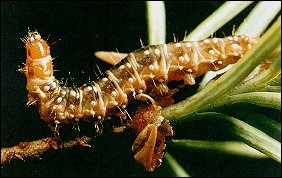
\includegraphics[width=\linewidth, keepaspectratio=1]{wbw-cov.jpg}
    % \end{figure}
    \end{minipage}
    In larger numbers, the budworms are too numerous for predation by birds to
    effectively control, and their population can grow explosively. Your team
    is part of an effort coordinated by United States and Canadian forest
    management agencies to determine whether this is likely to happen and, if
    appropriate, to recommend countermeasures and estimate their cost. Other
    important information is available to your group via the
    \emph{Conservation Algorithm Network of Vast Aquatic Significance}, known
    more commonly as C.A.N.V.A.S.

\subsection*{Useful facts and assumptions}
\vspace{-2.8ex}

    \begin{compactitem}

        \item Forest service personnel have collected data on the budworm
        population during the first few weeks of the season.

        \item Faced with limited scientific information,
        your team has to construct a model for how the budworm population over
        the course of a single season (May 1 to October 31). Based on past
        studies, your group has decided to try to fit the data from the forest
        service on the rate of budworm growth to one of two models,
        using vector projection. Your choice of which model is best will be
        based on a comparison of residual vectors.

        \item If at any time during the season the budworm population exceeds
        the critical threshold, the forest will largely be destroyed. However,
        if pesticides can be applied before the population growth rate ever
        reaches 80\% of its maximum, the budworms can be killed en masse and
        the forest will be saved.

        \item The pesticide is very effective, but it is expensive to apply.
        Human workers must spray the trees by hand. It cannot be dropped
        cheaply from the air. It is possible that the cost will be too great
        for the agencies to support a pesticide intervention, which your team
        should anticipate if appropriate.

    \end{compactitem}

\newpage

    Your team must now pull together all of its ideas to model the budworm
    population and determine whether a pesticide intervention will be required
    to save the forest, and if so, whether it will be cost-effective. Once you
    finish your calculations, your team should write a professional report
    restating the problem and summarizing your work and your findings. The
    crappie mission is critical and there's no room for mistakes. A rough
    report just won't do. Thus, your report must contain at least one
    meaningful, carefully labeled graph that adds something to the argument
    your team is making. You should report all answers with three significant
    digits.

% \newpage

\subsection*{Report guidelines}
\vspace{-2.8ex}


\begin{compactdesc}
    \item[Preliminary check-in:] Thursday/Friday, November 16--17, with your
    instructor at a scheduled time.
    \item[Final report due:] Wednesday, November 29, at the beginning of
    class, in Canvas.
    \item[Group evaluations due:] Wednesday, November 29, by 11:59pm, in
    Canvas.
    \item[Final interview:] Thursday/Friday, November 30--December 1, with your
    instructor at a scheduled time.
    \item[Late papers/group evaluations:] will not be accepted.
\end{compactdesc}

\subsection*{Preliminary check-in and final interview meetings}
\vspace{-2.8ex}

Your group turns in one report and everyone in the group gets the same grade
for the Written Report section for this project. The Written Report accounts
for $35\%$ of your Project 1 grade.  The rest of your score ($65\%$) is earned
during the Preliminary Check-in and Final Interview meetings with your
instructor. In these meetings, you will answer a question regarding the
development of the report's results to demonstrate your participation in the
project.  You are expected to participate in the project, understanding both
the solution to the problem and the process by which it was obtained.

\subsection*{Written report}
\vspace{-2.8ex}

Use Microsoft Word or another suitable word processor. \textbf{Type all equations},
using (for example) the Microsoft Equation Editor built into Word and standard
mathematical notation. Use RStudio to make all graphs. Graphs must include
proper axis labels. Group members' names and class section (01, 02, or 03)
must be clearly visible on the front page of your report. Margins will not
exceed 1 inch and lines are to be no more than 1.5-spaced.

Reports will be self-contained, i.e., the reader will not need prior knowledge
or understanding of the problem to understand your report. Your calculations
and conclusions will be explained in detail, as befits a professional report.
This report will be used by people of varying mathematical background, so do
your best to keep your report at a level accessible to the widest possible
audience (in other words, try to write for the general public whenever
possible). Your explanation and presentation are as important as the
mathematics, but of course your mathematical analysis must be clear, complete,
and correct. It should go without saying that your grammar, punctuation, and
spelling will be flawless.

\subsection*{Group evaluation}
\vspace{-2.8ex}

Every group member is required to submit to their instructor an informal group
evaluation \emph{the same day the reports are due}. The evaluation is at most
a short paragraph about how well the group worked together. The evaluation
\emph{must} include your estimate of the share of the project work that you
feel each group member did, expressed as a percentage (e.g.~33\%/33\%/33\% or
40\%/30\%/30\%, etc.). These percentages must add to 100\%---or 99\% is close
enough. These evaluations will be held in confidence, and used at the end of
the semester, if necessary, to adjust final grades.

\subsection*{A word to the wise}
\vspace{-2.8ex}

This project counts for 10\% of your final grade. Please make sure that
your report's qualities of clarity, completeness, and correctness
reflect your best abilities. Please carefully read all the instructions
and resources provided.

\end{document}



\end{document}
